\documentclass{article}

\usepackage[utf8]{inputenc}
\usepackage[T1]{fontenc}
\usepackage{lipsum}
\usepackage{graphicx}
\usepackage{amsmath}
\usepackage[margin=1in]{geometry}
\usepackage{titlesec}
\usepackage{enumitem}

\titleformat{\section}
{\LARGE\bfseries}{\thesection}{1em}{}

\titleformat{\subsection}
{\Large\bfseries}{\thesection}{1em}{}

\begin{document}
\pagestyle{empty}
\section*{GRASP}
\large

\subsection*{Introduzione}
\large
Obiettivi:
\begin{itemize}
    \renewcommand{\labelitemi}{-}
    \itemsep0em
    \item Definire che cos'è un pattern
    \item Comprendere quali siano i pattern che contraddistinguono GRASP
\end{itemize}
Il capitolo concentra la propria descrizione su quali metodi debbano essere attuati, affinchè il sistema software possa essere considerato di buona qualità. Fino ad ora il processo adottato per la creazione di una soluzione conforme ai requisiti funzionali, pone le proprie fondamenta sul concetto di \textit{object design}, costituita da un insieme di passi consecutivi.\vspace*{14pt}\\
Tuttavia, questa breve descrizione non è di gran auspicio, dato che in qualsiasi step che la compone, potrebbero sollervarsi problematiche e \textit{design smells}, peggiorando la qualità del software.\vspace*{14pt}\\
Per cui è necessario uno strumento in grado di illustrare singole direttive capaci di approcciare un metodo empirico ad una progettazione legata agli oggetti, eliminando ogni grado di incertezza. Ciò è possibile attraverso l'implementazione dei \textit{pattern} del modello \textit{GRASP}.

\subsection*{Responsability}
\large
UML definisce una \textbf{responsabilità} come un \textit{contratto oppure un obbligo di un classificatore}; per cui, brevemente, rappresenta un vincolo comportamentale di una certa istanza di classi software. Tipicamente sono suddivise in due macro-aree, le quali si contraddistinguono in:
\begin{itemize}[label={-}]
    \itemsep0em
    \item \textit{Doing}, responsabilità che a loro volta includono certi atteggiamenti, come operare per stessi termini, ossia creare un'istanza o processare un calcolo internamente, inizializzare un'azione per ulteriori oggetti oppure controllare e gestire attività di altre istanze
    \item \textit{Knowing}, in cui responsabilità simili illustrano una serie di comportamenti, quali, conoscere i dati incapsulati ad un specifico oggetto, apprendere a quali oggetti sia relazionato oppure comprendere quali elementi possano derivare per proprie azioni
\end{itemize}
Per cui in breve le due tipologie possono essere riassunte come segue; \textit{doing responsabilities} permettono la realizzazione di computazioni algoritmiche, mentre \textit{knowing responsabilities} prevedono di apprendere le informazioni interne ad ogni istanza di riferimento.\vspace*{14pt}\\
Una responsabilità non può essere paragonata ad un metodo, ma un metodo implementa responsabilità. Quest'ultimo inciso indica una caratterizzazione sottile, la quale può essere considerata mediante un \textit{activities diagram}. Si prenda come esempio il diagramma posto all'interno del capitolo \textit{design goal}; l'attore pur di apprendere il totale della spesa effettuata, demanda la richiesta alla classe \textit{saleManager}, il quale a sua volta, pur di ottenere l'informazione, reclama il valore alla classe \textit{sale}, contenente l'insieme di attributi e funzioni in grado di rispondere alla domanda.\vspace*{14pt}\\
Nonostante rappresenti una raffigurazione di estrema semplicità, si nota l'affermazione precedente, ossia i metodi implementano responsabilità, delegando \textit{vincoli comportamentali} ad una sequenzialità di istanze, reperendo tutto il necessario.\vspace*{14pt}
\subsection*{GRASP}
\large
\textit{GRASP} è l'acronimo di \textit{General Responsability Assignment Software Pattern}, ossia descrive i principi fondamentali della progettazione ad oggetti e permette l'assegnazione di responsabilità, detti \textit{patterns}. Spesso è utilizzato per implementare gli aspetti salienti di \textit{RDD} ma garantendo una solida costruzione sui principi cardine. In ingegneria del software il paradigma introdotto è considerato come l'artefice del conseguimento in sistemi software di spessore, poichè permette di analizzare e comprendere gli elementi essenziali nella progettazione ad oggetti, applicando un approccio metodico, razionale e improntato alla massima espressività.\vspace*{14pt}\\
Prima di illustrare i differenti apici su cui è posto, è bene definire l'etimologia dell'espressione \textit{pattern}.\vspace*{14pt}\\
\textit{Definizione informale}\\
Un \textbf{pattern} è una soluzione generale ad un problema ricorrente.\vspace*{14pt}\\
Come da considerazione descritta dall'architetto Alexander, un qualsiasi \textit{pattern} illustrato considera un problema che occorre frequentemente all'interno di un ambiente, ed è capace di associarne una soluzione, la quale può essere adottata con lo stesso metodo per risolvere correntemente la problematica. Riassumendo quanto detto, tramite il termine pattern, un problema ricorrente di medesima natura può essere risolto dalla stessa soluzione precedente.\vspace*{14pt}\\
Favorendo un'ulteriore chiave di lettura dal teorico Larman, un \textit{pattern}, per maggiore semplicità, rappresenta una descrizione nominativa di un problema e della sua soluzione correlata, indicando quando e come applicarla in nuovi contesti.\vspace*{14pt}\\
Introdotto il concetto su cui fonda l'intero contesto è possibile definire ora quali siano i pattern che contraddistringuono il modello \textit{GRASP}.

\subsection*{Patterns}
\large
Di seguito sono riportati i \textit{patterns} principali che contraddistinguono il modello \textit{GRASP}, in cui è attuata una suddivisione tra la definizione del problema e della soluzione correlata.\vspace*{14pt}\\
\textbf{Information expert}\vspace*{7pt}\\
\textit{Problema}\\
Come assegnare propriamente responsabilità all'istanze delle classi software?\vspace*{7pt}\\
Durante la fase di \textit{project design} potrebbero essere definite un numero sempre più elevato di responsabilità tra le classi, e lo stesso processo esecutivo potrebbe richiedere una quantità crescente di vincoli comportamentali. Buona pratica consiste nell'assegnare le \textit{responsabilities} tra \textit{software classes} durante la modellazione dell'interazioni tra oggetti; 
ossia si allude alla progettazione di \textit{interaction diagram}, in cui risulta ben visibile quali siano gli obiettivi e come essi possano essere soddisfatti. Se viene garantita questa possibilità allora il sistema software è caratterizzato da elevata \textit{reusability}.\vspace*{14pt}\\ 
\textit{Soluzione}\\
La soluzione consiste nella sistematizzazione della classe software che acquisisca la responsabilità. L'espressione riportata indica che l'assegnamento di responsability dovrebbe accadere nei confronti di classi già esistenti, scegliendo tra quelle che comprendano il numero maggiore di risorse necessarie (\textit{si ricordi nuovamente il parallelismo con l'esempio della sezione design goal, in cui la responsabilità di rispondere alla richiesta del costo totale della spesa è delegata alla classe sale, poichè contiene al suo interno tutte le informazioni principali di riferimento}).\vspace*{14pt}\\
\textit{Caso di studio}\\
Si analizza la progettazione di una soluzione in grado di poter attribuire la spesa finale che l'attore dovrà sostenere pur di acquisire i prodotti selezionati.
\begin{center}
    \includegraphics*[width=0.9\textwidth]{foto 1.png}
\end{center}\vspace*{7pt}
Secondo il pattern presentato, occorre osservare la classe software che contenga il numero maggiore di informazioni congrue alla richiesta del \textit{totale spesa}, analizzando sia design model che domain model.\vspace*{7pt}\\
Tuttavia assumendo della totale mancanza di \textit{interaction diagram}, l'unico diagramma in grado di illustrare ciò che sia necessario per implementare il vincolo comportamentale consiste in un \textit{class diagram}, come riportato nell'esempio. Per cui la \textit{responsabilità} sarà delegata alla classe software \textit{Sale}, poichè detiene il numero maggiore di risorse riconducibili alla realizzazione dell'obiettivo.\vspace*{7pt}\\
Procedendo gradualmente, si verifica la necessità che la classe \textit{Sale} debba delegare comportamenti specifici affinchè possa apprendere la \textit{lista dei prodotti acquistati} e i \textit{subtotals} di riferimento. Proprio per questa ragione, oltre al \textit{class diagram}, è riportata la raffigurazione di un \textit{sequence diagram}. La ragione principale è dovuta alla chiara visualizzazione dell'obiettivo del \textit{pattern Information Expert}, dove la classe \textit{Sale} rappresenta l'\textit{esperto} in grado di assimilare tutte le informazioni del contesto, divenendo l'elemento del modello con il numero maggiore di informazioni necessarie.\vspace*{14pt}\\
\textbf{Creator}\vspace*{7pt}\\
\textit{Problema}\\
Come scegliere chi dovrebbe essere il responsabile della creazione di nuove istanze di classi software?\vspace*{7pt}\\
La creazione di oggetti è una delle pratiche più comuni di un linguaggio legato al paradigma degli oggetti. Conseguentemente, sarebbe utile individuare un principio in grado di stabilire una responsabilità affine all'istanze di oggetti. Una correlazione corretta della responsability potrebbe alludere ad una maggiore chiarezza sintattica e alla massimizzazione dell'\textit{incapsulazione} e della qualità \textit{reusability}.\vspace*{14pt}\\
\textit{Soluzione}\\
Adoperando una semplificazione semantica, l'assegnazione della responsabilità alla classe B, autrice della creazione di un'istanza della classe A, è corretta se rispettata almeno una delle condizioni seguenti:
\begin{itemize}[label={-}]
    \itemsep0em
    \item B aggrega, ossia contiene o compone, oggetti di A 
    \item B contiene oggetti di A 
    \item B utilizza fortemente oggetti di A
    \item B è in possesso di tutti i dati necessari per poter richiamare la funzione della classe software A, banalmente ha a disposizione tutti gli attributi sufficienti per il metodo di destinazione
\end{itemize}
Nel caso più classi dovessero rispettare le condizioni elencate, si tende a premiare effettività che comprendano le prime due caratteristiche illustrate.\vspace*{14pt}\\
\textit{Caso di studio}\\
Tale sezione domanda chi dovrebbe essere il responsabile della creazione di istanze di \textit{SaleLineItems}. Secondo il pattern \textit{Creator}, dovrebbe essere scelta la classe che compone, aggrega oppure contiene le istanze di \textit{SaleLineItems}. Dato che \textit{Sale} rappresenta una classe che contiene più istanze di \textit{SaleLineItems}, potrebbe essere un buon candidato a cui assegnare la \textit{responsabilità di creazione}.\vspace*{7pt}
\begin{center}
    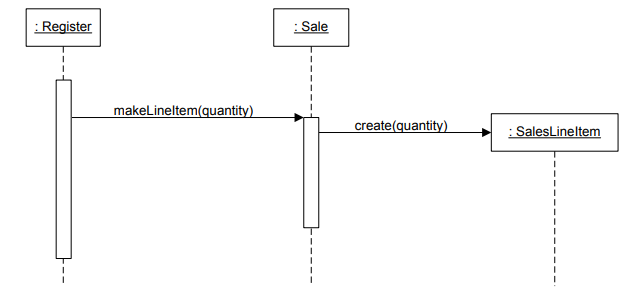
\includegraphics[width=0.9\textwidth]{foto 2.png}
\end{center} 
Nuovamente, il contesto in cui le responsabilità siano decise e assegnate avviene durante la fase di progettazione dell'\textit{interaction diagram}.\vspace*{14pt}\\
\textbf{Controller}\vspace*{7pt}\\
\textit{Problema}\\
Come scegliere quale oggetto debba ricevere e coordinare un'operazione del sistema software?\vspace*{7pt}\\
Differenti sono i \textit{patterns} valutativi in cui possono essere presi in considerazione candidati piuttosto simili fra loro, in relazione alle classi poste all'interno del domain model. Il termine \textit{controller} è adottato proprio per esprimere una soluzione al problema; \textit{classi di controllo} potrebbero divenire uno strato posto tra classi di alto livello, quindi affini alla logica algoritmica, e classi di basso livello, per cui in relazione ad una raffigurazione dell'entità usufruibili dall'utente finale. L'utilizzo di uno scudo sovrapposto permette di isolare elementi dinamici, proprio come \textit{user interface}, i quali non devono mai interagire con classi prettamente legate allo sviluppo di metodi basici, corrispondendo appieno al \textit{Liskov Substitution Principle} (\textit{si ricordi l'activity SaleManager all'interno del capitolo design goal, posto in mezzo all'attività UI e sale}).\vspace*{14pt}\\
Concludendo, un controller non rappresenta un'interfaccia finale con cui utenti possano interagire, ma definisce l'architettura comportamentale del sistema software dinnanzi alla ricezione e gestione di eventi.\vspace*{14pt}\\
\textit{Soluzione}\\
Come già accennato dall'introduzione del problema, porre responsabilità relative alla gestione di eventi del sistema dovrebbe avvenire nei confronti di interfacce create appositamente per la manipolazione di trasferimenti di dati e richiesta di informazioni. L'assegnazione richiede che siano rispettate almeno una delle seguenti condizioni, quali:
\begin{itemize}[label={-}]
    \itemsep0em
    \item Una classe simile rappresenta il cosiddetto \textit{root object}, ossia l'elemento che il software in questione provvede ad interpellare con maggiore frequenza, spesso illustrato come il sottosistema che contiene tutte le \textit{variazioni comportamentali di facciata}, ossia la totalità di funzioni che una \textit{GUI} implementata possa richiedere alle \textit{high level classes}, mediante un \textit{controller}
    \item La classe è denominata tramite il nominativo di riferimento al \textit{caso d'uso} modellato, in cui è anteposta la nomenclatura \textit{Handler}, \textit{Controller} oppure \textit{Session}. Per cui, attuando una semplificazione, qualora adottato \textit{UseCaseNameController} esso sarà il punto cardine su cui tutti gli eventi del caso d'uso faranno riferimento
\end{itemize}\vspace*{7pt}
\textbf{Low Coupling}\vspace*{7pt}\\
\textit{Problema}\\
Come stabilire dinamiche che scoraggino \textit{elevata dipendenza} e \textit{impatto modellativo}, affinchè si possa massimizzare il \textit{riutilizzo}?\vspace*{7pt}\\
\textbf{Coupling} è una misura di quanto un elemento sia fortemente connesso o meno rispetto a possibili corrisposti. Per elemento si intende un insieme di caratterizzazioni, come classi, sistemi oppure sottosistemi. Per cui un elemento con un \textit{low coupling}, ossia un basso layer di accoppiamento, non è dipendente da un numero crescente di entità, mentre in maniera opposta un elemento è detto \textit{strong coupling} qualora sia artefice di \textit{contesti dipendenti}. Si nota nuovamente la centralità delle \textit{dipendenze} e delle problematiche derivanti da esse, totalmente contrarie rispetto all'obiettivo del pattern illustrato, tra cui:
\begin{itemize}[label={-}]
    \itemsep0em
    \item Cambiamenti suscitano modifiche locali delle classi, situazione contraria rispetto all'\textit{OOP}, ossia \textit{Open Closed Principle}
    \item Maggiore complessità nell'intento di isolare elementi software
    \item Maggiore complessità relativa al \textit{riutilizzo} dato che l'implementazione delle classi ha portato ad un numero elevato di dipendenze, producendo un effetto a cascata
\end{itemize}\vspace*{7pt}
\textit{Soluzione}\\
Assegnare responsabilità affinchè sia mantenuto basso livello di accoppiamento.\vspace*{14pt}\\
\textit{Caso di studio}\\
L'obiettivo consiste nella creazione di un'istanza della classe \textit{Payment} affinchè sia usufruibile dalla classe \textit{Sale}.\vspace*{7pt}
\begin{center}
    \includegraphics*[width=0.7\textwidth]{foto 3.png}
\end{center} 
Il pattern \textit{Creator} suggerisce che sia \textit{Register} la classe artefice della creazione di istanze di \textit{Payment}, rappresentando un nodo intermedio in grado di inoltrare tutto il necessario alla classe \textit{Sale}. In questo contesto, una soluzione simile mantiene un livello di accoppiamento piuttosto basso; tuttavia, qualora a \textit{Register} siano attribuite più responsabilità potrebbe provocare un aumento del livello di accoppiamento, causando un accumolo di \textit{dipendenze}.\vspace*{14pt}\\
\textbf{High Coesion}\vspace*{7pt}\\
\textit{Problema}\\
Come rendere gli elementi del modello comprensivi e maneggevoli, i quali possano essere anche un termine di supporto per il pattern valutativo \textit{Low Coupling}?\vspace*{14pt}\\
Il problema potrebbe essere riassunto semplicemente in come mantenere una complessità modellativa costante e manipolabile. Similmente al pattern \textit{Low Coupling}, è introdotta una misura dedicata a tale tipologia di risoluzione, la \textit{coesione}. La \textit{functional cohesion} è la capacità adottata per distinguere il grado di correlazione di una \textit{responsabilità} rispetto ad un'ipotetica associazione ad elementi del dominio, come classi o sistemi. Classi con un livello elevato di responsabilità, non indicano una quantità operativa consistente, ma definiscono un elevato layer di coesione. Per cui l'assegnazione di responsabilità non va di pari passo rispetto all'operatività inclusa all'interno dell'elemento del dominio, anzi classi con basso livello di coesione illustrano situazioni sormontate dalla quantità di funzionalità da eseguire. I difetti relativi a quest'ultimo passaggio sono descritti come segue:
\begin{itemize}[label={-}]
    \itemsep0em
    \item Difficile comprensione e manutenzione
    \item Il principio \textit{reusable} non è attuabile
    \item Piuttosto sensibili a modifiche, piccole variazioni potrebbero provocare enormi cambiamenti
\end{itemize}\vspace*{7pt}
\textit{Soluzione}\\
Attribuire responsabilità affinchè sia mantenuta elevata coesione.\vspace*{14pt}\\
\textit{Caso di studio}\\
Lo stesso caso di studio analizzato in \textit{Low Coupling} può essere inizializzato per \textit{High Coesion}. Come già illustrato, il fatto che la classe \textit{Register} sia responsabile della creazione delle due istanze rappresenta una scelta accettabile, all'interno del contesto. Tuttavia se si dovesse continuare a responsabilizzare la classe \textit{Register} per ogni futura operazione del sistema software, renderà l'elemento di difficile comprensione e di totale mancanza di coesione tra le funzionalità implementate. Per cui è necessario introdurre un'ulteriore effettività, sempre espressa mediante un \textit{interaction diagram}, la quale proponga un passaggio intermedio, il quale può essere propriamente considerato come definito dal pattern \textit{Indirection}.
\begin{center}
    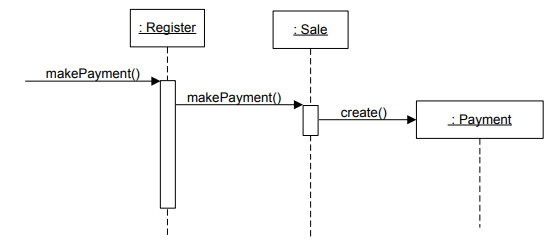
\includegraphics[width=0.6\textwidth]{foto 4.png}\vspace{7pt}
\end{center}
\textbf{Indirection}\vspace*{7pt}\\
\textit{Problema}\\
Come assegnare responsabilità affinchè sia possibile ovviare ad un accoppiamento tra due o più elementi, e come attuare il processo opposto al coupling per supportare un riutilizzo potenzialmente maggiore?\vspace*{14pt}\\
In questo contesto gioca un ruolo fondamentale l'aspetto della \textit{pura invenzione}, o meglio definito \textbf{pure fabrication}. Non riguarda la creazione di elementi senza un rigore modellativo e logico, ma attua un iter di step affinchè sia necessaria una figura che possa sia elaborare funzioni di \textit{coupling} che di \textit{de-coupling}. Dopo aver analizzato tutte le classi presenti a cui applicare tale responsabilità, se non individuate caratteristiche che possano mantenere un livello elevato di coesione e nessuna di esse definisca un \textit{Information Expert}, è necessario introdurre entità, mediatori che possano allineare e disallineare dipendenze tra classi.\vspace*{14pt}\\
\textit{Soluzione}\\
Le responsabilità dovrebbero essere assegnate ad un \textit{intermediario}, ossia un mediatore tra differenti componenti del sistema software che non siano direttamente dipendenti.\vspace*{14pt}\\
\textbf{Protected Variations}\vspace*{7pt}\\
\textit{Problema}\\
Come progettare elementi affinchè le loro instabilità non siano d'impatto su altri componenti della modellazione?\vspace*{14pt}\\
Il pattern \textit{Protected Variations} è essenzialmente al pari del principio \textit{OCP}, \textit{Open Closed Principle}, il quale afferma che una classe dovrebbe essere aperta a nuove funzionalità ma non al cambiamento di metodi già implementati. Per cui rimanda all'uso di astrazioni modellative qualora vi sia la netta necessità, come le interfacce, affinchè cambiamenti legati a \textit{low level classes} non riguardino metodi legati alla logica algoritmica. A favore di quanto detto, si adopera in questa tematica la \textit{legge di Demetra}; essa formula il pretesto secondo cui una classe dovrebbe interagire, mediante metodi, chiamate alle funzioni interessate oppure alla creazione di istanze, solamente con entità di cui abbia lo stretto collegamento. Semplicimente, vanificando il contesto teorico, la classe dovrebbe invocare procedure di cui abbia tutto il necessario, evitando di gestire dipendenze superflue.\vspace*{14pt}\\
\textit{Soluzione}\\
La soluzione prevede l'identificazione precedente di elementi soggetti ad instabilità, modellando interfacce che circondino l'insieme di entità dannose, dove un profondo cambiamento non intralci ulteriori oggetti. Concludendo, una piccola nota aggiuntiva, consiste che il termine \textit{interfaccia} sia adoperato nel suo più ampio senso etimologico, principalmente a livello di astrazione piuttosto che implementativo, come accadrebbe per linguaggi orientati al paradigma degli oggetti, stabilendo una struttura \textit{flessibile} improntata ad adeguarsi a possibili modifiche.
\end{document}